\chapter{Arduino}\label{analysis:arduino}
Arduino was created by the Interaction Design Institute Ivrea (Italy), by Massimo Banzi and David Cuartielles. They were looking for an easy and cheap way for students, who study design, to integrate micro controllers into their projects\cite{arduino:hist}. Both the board and the programming language was based on the works of Hernando Barragán, one of Massimo Banzi master thesis students \cite{Wiring:thesis}

\section{The hardware components}
Arduino is a single-board micro-controller, see figure \ref{fig:Arduino}.
A board consists of open source hardware, which is designed around an 8-bit Atmel AVR micro-controller. Arduino boards varies in sizes. Arduino Uno board for example, has a max width of 2.1'' (5,33cm) and a length of 2.7'' (6,86cm).  \\

\par
\raisebox{-.5\height}{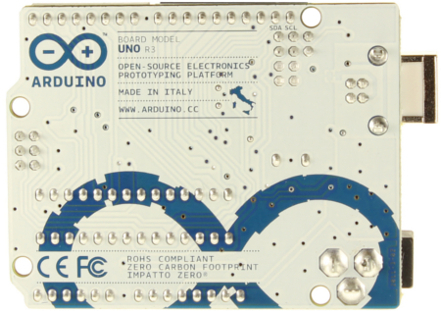
\includegraphics[width=6.5cm]{billeder/ArduinoUno_R3_Back_450px.jpg}}
\hfill
\raisebox{-.5\height}{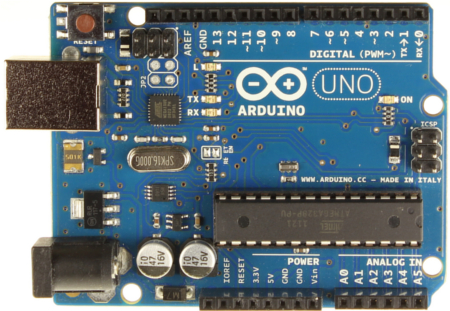
\includegraphics[width=6.5cm]{billeder/ArduinoUno_R3_Front_450px.jpg}}
\begin{figure}[H]
\caption{Picture of back- and fronside of the Arduino board \cite{Arduino_board_pics}}
\label{fig:Arduino}
\end{figure}
\par

\subsection*{Specifications}
\begin{figure}[hbtp]
\centering
\begin{tabular}{|c|c|}
\hline 
Microcontroller & ATmega328 \\ 
\hline 
Operating Voltage & 5V \\ 
\hline 
Input Voltage (recommended)	 & 7-12V \\ 
\hline 
Input Voltage (limits) & 6-20V \\ 
\hline 
Digital I/O Pins & 14 (of which 6 provide PWM output) \\ 
\hline 
Analog Input Pins & 6 \\ 
\hline 
DC Current per I/O Pin & 40 mA \\ 
\hline 
DC Current for 3.3V Pin & 50 mA \\ 
\hline 
Flash Memory & 32 KB (ATmega328) of which 0.5 KB used by bootloader \\ 
\hline 
SRAM & 2 KB (ATmega328) \\ 
\hline 
EEPROM & 1 KB (ATmega328) \\ 
\hline 
Clock Speed & 16 MHz \\ 
\hline 
\end{tabular} 
\caption{Hardware specifications for the Arduino Uno}
\end{figure}


The board provides some input and output possibilities. However these vary depending on the board, though the Arduino Uno have 14 digital I/O and 6 analog inputs. The I/O functions are placed on top of the board, are freely accessible, and consist of 0.1'' female headers. Besides the I/O there is also a Power connector, which almost in all cases require 5 volt DC. There is a USB connection on the board, so that processing data to the micro-controller is possible, though it is shown as a virtual com-port on the connected computer. However, on older boards, instead of the USB connection, a RS232 were used for serial communication. 

On the board there is a LED diode which is connected to the digital pin 13. When this diode is set to ``HIGH'' it will be turned on, and if its value is ``LOW'' it turns off. Besides the LED diode, there is also a reset button. If the button is pressed the micro-controller is reset. \\

The specifications which are important to take into consideration with regards to designing a programming language aimed at the Arduino platform is the flash memory, the main memory(SRAM) and the cpu speed, the most limiting factor to take into consideration is the amount of RAM, the larger and more complex data structures which are implemented, the bigger the risk of running out of memory while executing a program. Although this is not limited to developing for the Arduino platform, it is certainly a larger factor, then when developing for desktop computers.\\

Another factor is the flash memory, the space available for the program, the smallest example code, the Arduino blink sketch, uses 1084 bytes, and the FooBar example, code example \ref{lst:second_syntax_example}, uses 4456 bytes, so if a language is cramped with lots of fancy features and unnecessary features, it will quickly run out of space. For instance with more complex languages like C\#, a simple hello world program uses 5120 bytes, and they can quickly run in the hundreds or thousands of kilobytes. This is even more important to remember, when one takes into account that there are many different Arduino configurations, and the language have to function on all of them, then Arduino Nano for instance only have 16 KB of memory, and there are Arduino clones by other manufactures with even less.  

\subsection*{Components}
Now what makes Arduino such a good platform for beginners to learn to code, is the fact that it is really easy to hook up the Arduino platform, to a wide array of components, to make it possible for the Arduino to interact with the real world.


\begin{itemize}
\item[] \textbf{LED's} They come in all size, shapes and colors, ranging from small pin size single color LED's, to large multi color led displays.
\begin{figure}[hbtp]
\centering
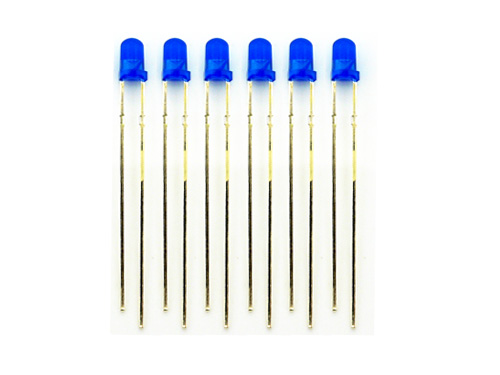
\includegraphics[width=5cm]{billeder/led.jpg}
\caption{3mm blue led}
\end{figure}
\item[] \textbf{Sensors} These are some of the main components behind the Arduino success, they give the Arduino the ability to sense its surroundings, for instance the temperature of the room, whether the light is turn on, even advanced sensors like humidity or gas.
\begin{figure}[hbtp]
\centering
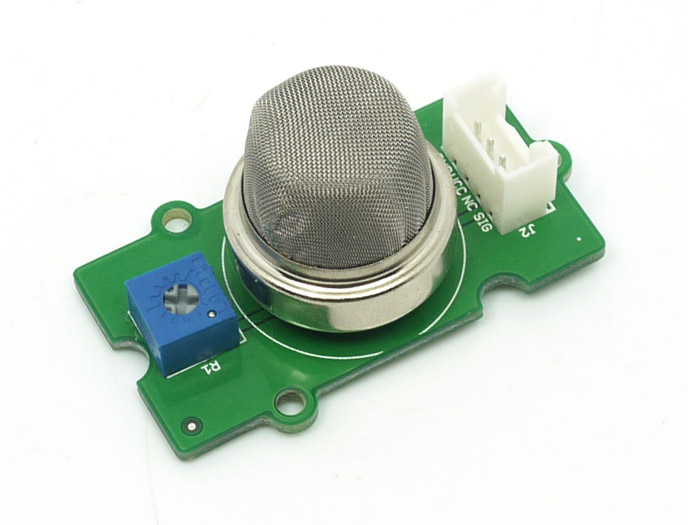
\includegraphics[width=5cm]{billeder/Sensor.jpg}
\caption{Gas sensor}
\end{figure}
\item[] \textbf{Motors} They give the Arduino the ability to manipulate its surrounding, and act on the informations obtained from the sensors. There are two kind of motors, normal motors which can just be turned on/off, they are great for powering wheels or tracks to allow it to move. There are stepper motors with it is possible to control the exact amount of rotation. And finally there is servos, which are precisely controlled motors much like the stepper motor, but much more precise.
\begin{figure}[hbtp]
\centering
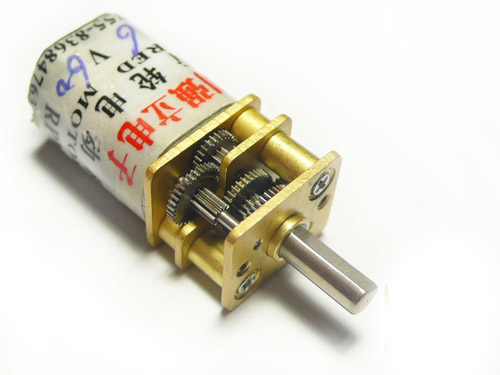
\includegraphics[width=5cm]{billeder/Motor.jpg}
\caption{Geared stepper motor}
\end{figure}
\item[] \textbf{Displays} There are a wide range of display available ranging from simple 2 line mono color LCD displays, all the way up to large OLED color and touch displays. 
\begin{figure}[hbtp]
\centering
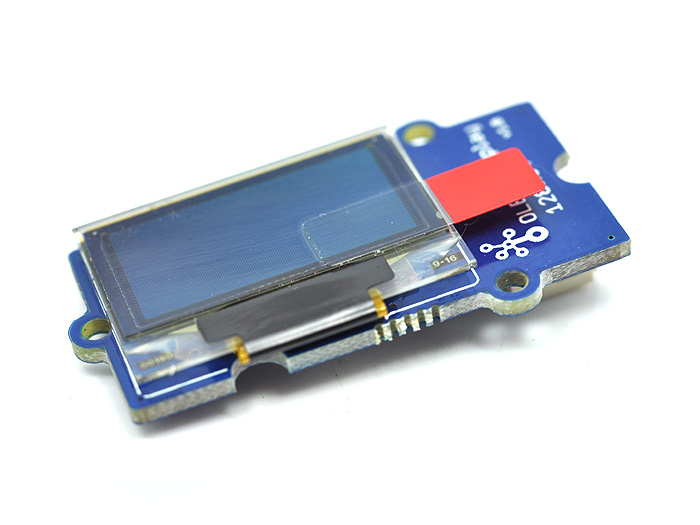
\includegraphics[width=5cm]{billeder/display.jpg}
\caption{OLED thuch display}
\end{figure}
\item[] \textbf{Communication} It is easy to hook up the Arduino with some form of communication allowing it to communicate with other devices either through, RF signals, bluetooth, WiFi, cellular or just plain old Ethernet connection.
\begin{figure}[hbtp]
\centering
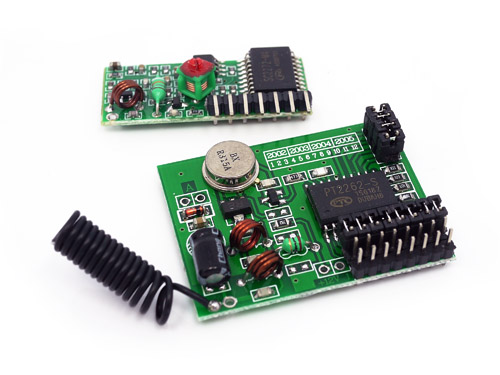
\includegraphics[width=5cm]{billeder/com.jpg}
\caption{RF transmitter and reciver}
\end{figure}
\item[] \textbf{Shields} Finally the last thing which makes the Arduino great is it modularity, in the form of shields. Shields are boards much like the Arduino it self, but they offer all the capabilities of the components mentioned above, but they do it in a way, which makes it possible for any one with out any electronics experience to use them, you just plug the shield on top of the Arduino board, and all the components need to are included.
\begin{figure}[hbtp]
\centering
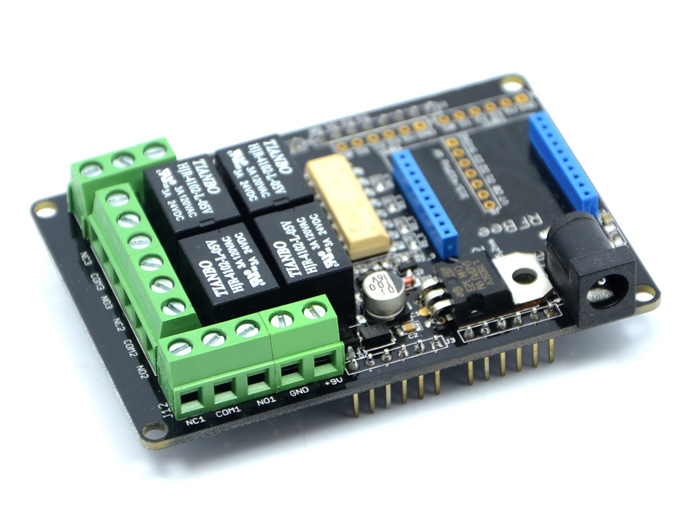
\includegraphics[width=5cm]{billeder/Shield.jpg}
\caption{Relay shield}
\end{figure}

\end{itemize}


